\part{Annexes} % (fold)
\label{prt:annexes}

	\chapter{Organigramme} % (fold)
		\begin{appendices}

		\label{chap:organigramme}
		%\clearpage
			\phantomsection
			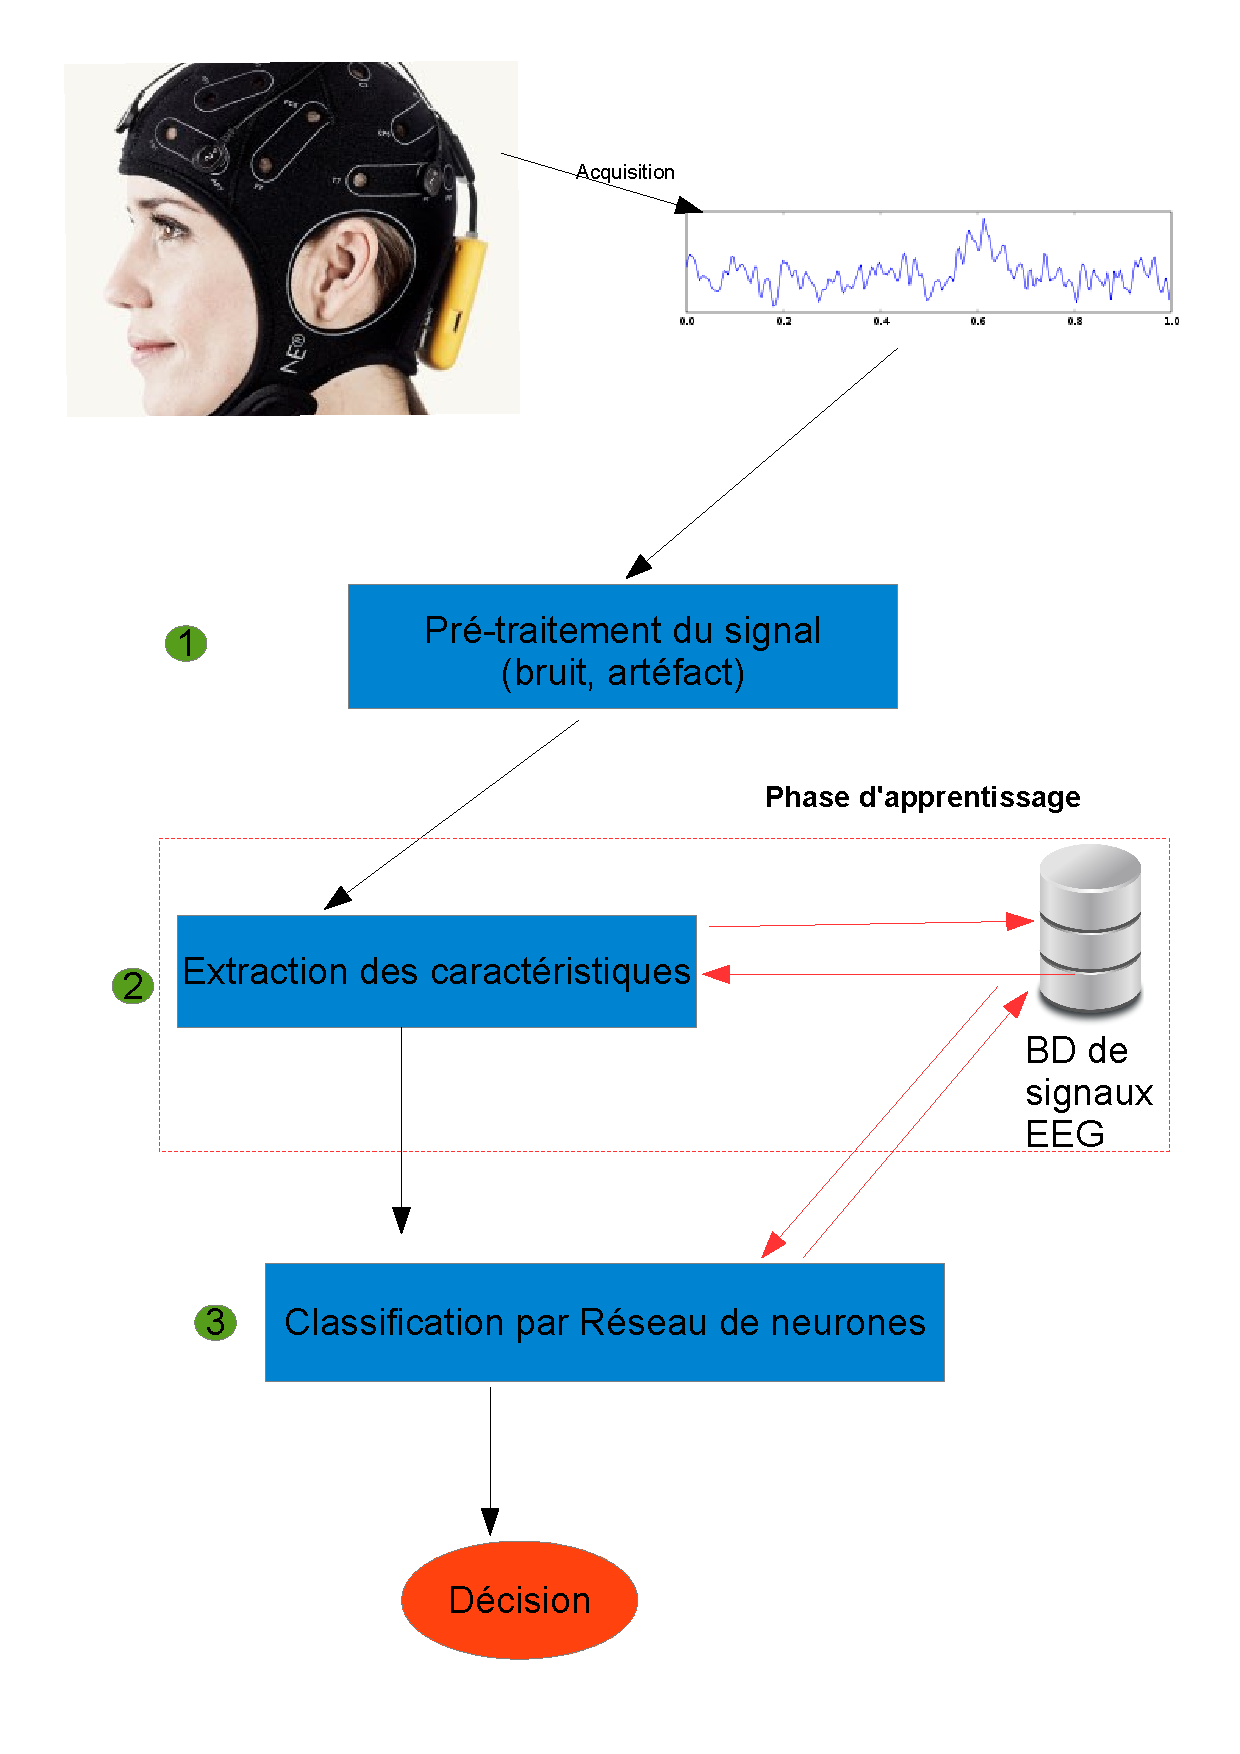
\includepdf[]{../organigramme/Organigramme_application.pdf}
		  \end{appendices}

	% chapter chapter_organigramme
	\chapter{Diagrammes de classes} % (fold)
		\begin{appendices}
			\label{chap:diag_class}
			%\clearpage
			%%%%%%%%%%%%%%%%%%%%%%%%%%%%%%%%%%%%%%%%%%%%
			\begin{figure}
			\centering
		    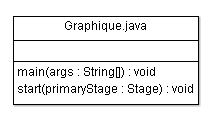
\includegraphics []{../diagramme_classes/charts.png} \\
		    \captionof{figure}{Classe Graphique}
			\label{fig_graph}
			\end{figure}
			%%%%%%%%%%%%%%%%%%%%%%%%%%%%%%%%%%%%%%%%%%%%
			\begin{figure}
		    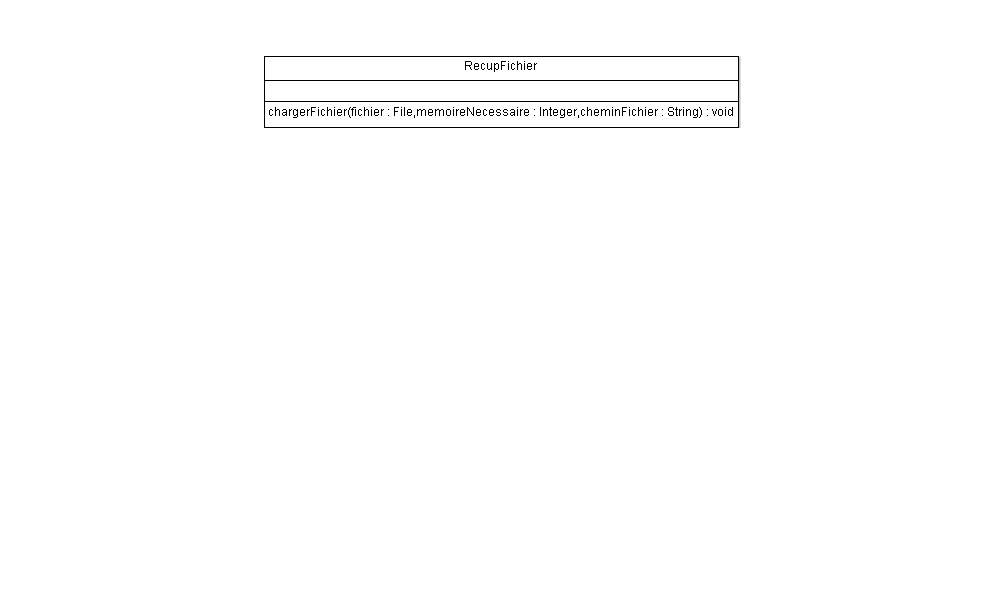
\includegraphics []{../diagramme_classes/donnees.png} \\
		    \captionof{figure}{Classe RecupFichier}
			\label{fig_donnees}
  			\end{figure}
			%%%%%%%%%%%%%%%%%%%%%%%%%%%%%%%%%%%%%%%%%%%%
			\begin{figure}
			\centering
		    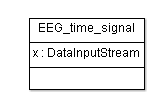
\includegraphics []{../diagramme_classes/eeg.png} \\
		    \captionof{figure}{Classe EEG\_time\_signal}
			\label{fig_eeg}
  			\end{figure}
			%%%%%%%%%%%%%%%%%%%%%%%%%%%%%%%%%%%%%%%%%%%%
			\begin{figure}
			\centering
		    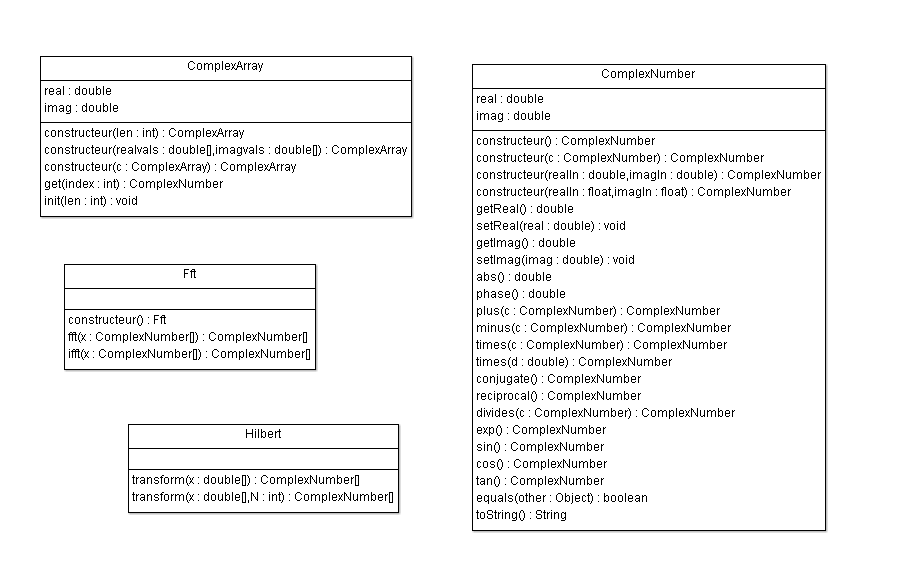
\includegraphics [scale=0.5]{../diagramme_classes/math.png} \\
		    \captionof{figure}{Classes pour les calculs mathématiques }
			\label{fig_math}
    		\end{figure}
			%%%%%%%%%%%%%%%%%%%%%%%%%%%%%%%%%%%%%%%%%%%%
			\begin{figure}
			\centering
		    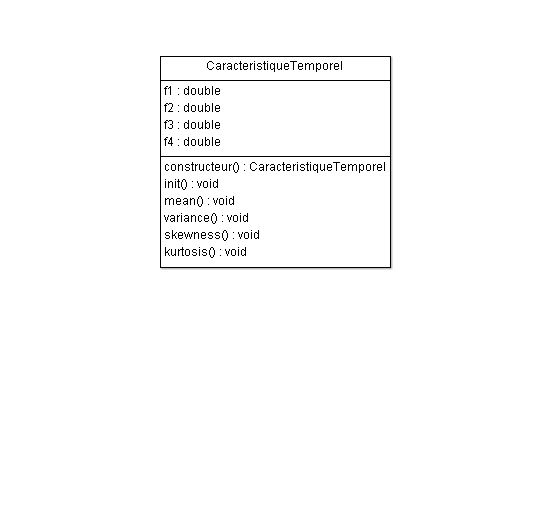
\includegraphics []{../diagramme_classes/neuron.png} \\
		    \captionof{figure}{Classe Caractéristique}
			\label{fig_neuron}
    		\end{figure}
			%%%%%%%%%%%%%%%%%%%%%%%%%%%%%%%%%%%%%%%%%%%%
			\begin{figure}
			\centering
		    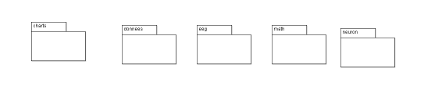
\includegraphics []{../diagramme_classes/packages.png} \\
		    \captionof{figure}{Packages composant l'application}
			\label{fig_pack}
    		\end{figure}
			%%%%%%%%%%%%%%%%%%%%%%%%%%%%%%%%%%%%%%%%%%%%
		\end{appendices}

	% chapter chapter_diag_class

% part part_annexes (end)